\section{Face Recognition}

Face recognition is an easy task for humans. Experiments in \cite{Tu06} have shown, that even one to three day old babies are able to distinguish between known faces. So how hard could it be for a computer? It turns out we know little about human recognition to date. Are inner features (eyes, nose, mouth) or outer features (head shape, hairline) used for a successful face recognition? How do we analyze an image and how does the brain encode it? It was shown by \href{http://en.wikipedia.org/wiki/David_H._Hubel}{David Hubel} and \href{http://en.wikipedia.org/wiki/Torsten_Wiesel}{Torsten Wiesel}, that our brain has specialized nerve cells responding to specific local features of a scene, such as lines, edges, angles or movement. Since we don't see the world as scattered pieces, our visual cortex must somehow combine the different sources of information into useful patterns. Automatic face recognition is all about extracting those meaningful features from an image, putting them into a useful representation and performing some kind of classification on them.

Face recognition based on the geometric features of a face is probably the most intuitive approach to face recognition. One of the first automated face recognition systems was described in \cite{Kanade73}: marker points (position of eyes, ears, nose, ...) were used to build a feature vector (distance between the points, angle between them, ...). The recognition was performed by calculating the euclidean distance between feature vectors of a probe and reference image. Such a method is robust against changes in illumination by its nature, but has a huge drawback: the accurate registration of the marker points is complicated, even with state of the art algorithms. Some of the latest work on geometric face recognition was carried out in \cite{Bru92}. A 22-dimensional feature vector was used and experiments on large datasets have shown, that geometrical features alone don't carry enough information for face recognition.

The Eigenfaces method described in \cite{PT91} took a holistic approach to face recognition: A facial image is a point from a high-dimensional image space and a lower-dimensional representation is found, where classification becomes easy. The lower-dimensional subspace is found with Principal Component Analysis, which identifies the axes with maximum variance. While this kind of transformation is optimal from a reconstruction standpoint, it doesn't take any class labels into account. Imagine a situation where the variance is generated from external sources, let it be light. The axes with maximum variance do not necessarily contain any discriminative information at all, hence a classification becomes impossible. So a class-specific projection with a Linear Discriminant Analysis was applied to face recognition in \cite{belhumeru97}. The basic idea is to minimize the variance within a class, while maximizing the variance between the classes at the same time (Figure \ref{fig:scatter_matrices}). 

Recently various methods for a local feature extraction emerged. To avoid the high-dimensionality of the input data only local regions of an image are described, the extracted features are (hopefully) more robust against partial occlusion, illumation and small sample size. Algorithms used for a local feature extraction are Gabor Wavelets (\cite{Wiskott97}), Discrete Cosinus Transform (\cite{Cardinaux2006}) and Local Binary Patterns (\cite{Ahonen04,Maturana09, Rodriguez2006}). It's still an open research question how to preserve spatial information when applying a local feature extraction, because spatial information is potentially useful information.

\subsection{Eigenfaces}

\lstset{language=matlab}

The problem with the image representation we are given is its high dimensionality. Two-dimensional $p \times q$ grayscale images span a $m = pq$-dimensional vector space, so an image with $100 \times 100$ pixels lies in a $10,000$-dimensional image space already. That's way too much for any computations, but are all dimensions really useful for us? We can only make a decision if there's any variance in data, so what we are looking for are the components that account for most of the information. The Principal Component Analysis (PCA) was independently proposed by \href{http://en.wikipedia.org/wiki/Karl_Pearson}{Karl Pearson} (1901) and \href{http://en.wikipedia.org/wiki/Harold_Hotelling}{Harold Hotelling} (1933) to turn a set of possibly correlated variables into a smaller set of uncorrelated variables. The idea is that a high-dimensional dataset is often described by correlated variables and therefore only a few meaningful dimensions account for most of the information. The PCA method finds the directions with the greatest variance in the data, called principal components.

\subsubsection{Algorithmic Description}

\label{ssection:pca_algorithm}

Let $X = \{ x_{1}, x_{2}, \ldots, x_{n} \}$ be a random vector with observations $x_i \in \mathbb{R}^{d}$.

\begin{enumerate}
	\item Compute the mean $\mu$
		\begin{equation} \label{eqn:pca_mean}
			\mu = \frac{1}{n} \sum_{i=1}^{n} x_{i}
		\end{equation}
	\item Compute the the Covariance Matrix $S$
		\begin{equation} \label{eqn:pca_cov}
			S = \frac{1}{n} \sum_{i=1}^{n} (x_{i} - \mu) (x_{i} - \mu)^{T}
		\end{equation}
	\item Compute the eigenvalues $\lambda_{i}$ and eigenvectors $v_{i}$ of $S$
		\begin{equation}  \label{eqn:pca_eigenvalues}
			S v_{i} = \lambda_{i} v_{i}, i=1,2,\ldots,n
		\end{equation}
	\item Order the eigenvectors descending by their eigenvalue. The $k$ principal components are the eigenvectors corresponding to the $k$ largest eigenvalues.
\end{enumerate}

The $k$ principal components of the observed vector $x$ are then given by:

\begin{equation} \label{eqn:pca_projection}
	y = W^{T} (x - \mu)
\end{equation}

where $W = (v_{1}, v_{2}, \ldots, v_{k})$. The reconstruction from the PCA basis is given by:

\begin{equation} \label{eqn:pca_reconstruction}
	x = W y + \mu
\end{equation}

The Eigenfaces method then performs face recognition by:

\begin{enumerate}
	\item Projecting all training samples into the PCA subspace (using Equation \ref{eqn:pca_projection}).
	\item Projecting the query image into the PCA subspace (using Listing \ref{eqn:pca_reconstruction}).
	\item Finding the nearest neighbor between the projected training images and the projected query image.
\end{enumerate}

Still there's one problem left to solve. Imagine we are given $400$ images sized $100 \times 100$ pixel. The Principal Component Analysis solves the covariance matrix $S = X X^{T}$, where ${size}(X) = 10000 \times 400$ in our example. You would end up with a $10000 \times 10000$ matrix, roughly $0.8 GB$. Solving this problem isn't feasible, so we'll need to apply a trick. From your linear algebra lessons you know that a $M \times N$ matrix with $M > N$ can only have $N - 1$ non-zero eigenvalues. So it's possible to take the eigenvalue decomposition $S = X^{T} X$ of size $N x N$ instead:
\begin{equation}
	X^{T} X v_{i} = \lambda_{i} v{i}
\end{equation}

and get the original eigenvectors of $S = X X^{T}$ with a left multiplication of the data matrix:

\begin{equation}
	X X^{T} (X v_{i}) = \lambda_{i} (X v_{i})
\end{equation}

The resulting eigenvectors are orthogonal, to get orthonormal eigenvectors they need to be normalized to unit length. I don't want to turn this into a publication, so please look into \cite{Duda2001} for the derivation and proof of the equations.

\ifx\python\undefined 
	\subsubsection{Eigenfaces in GNU Octave/MATLAB}
\else
 \subsubsection{Eigenfaces in Python}
\fi


\label{ssection:example_eigenfaces}

It's always useful to prototype algorithms before implementing them with OpenCV, because this gives you an idea what the solution looks like. I've used \href{http://www.gnu.org/software/octave/}{GNU Octave}/\href{http://www.mathworks.com}{MATLAB} and \href{http://www.python.org}{Python} with \href{http://www.scipy.org}{NumPy} (and \href{http://matplotlib.sourceforge.net/}{matplotlib}) in this document. Please compile the document version you prefer. I recently switched to Python, because OpenCV2 uses \href{http://www.scipy.org}{NumPy} arrays since OpenCV 2.3. This means: all algorithms using \href{http://www.numpy.org}{NumPy} play fine with OpenCV's Python bindings, that's great news! Full-blown \href{http://www.gnu.org/software/octave/}{GNU Octave}/\href{http://www.mathworks.com}{MATLAB} and Python environments are available at \url{https://github.com/bytefish/facerec}, including:
\begin{itemize}
	\item Preprocessing 
	\begin{itemize}
		\item Histogram Equalization
		\item Local Binary Patterns
		\item TanTriggs Preprocessing \cite{Tan10}
	\end{itemize}
	\item Feature Extraction
	\begin{itemize}
		\item Eigenfaces \cite{PT91}
		\item Fisherfaces \cite{belhumeru97}
		\item Local Binary Patterns Histograms \cite{Ahonen04}
	\end{itemize}
	\item Classifier
		\begin{itemize}
			\item k-Nearest Neighbor Model (with various metrics)
			\item Support Vector Machine \cite{Vapnik1998}
		\end{itemize}
	\item Cross Validation
	\begin{itemize}
		\item k-fold CV 
		\item Leave One Out CV
		\item Leave One Subject Out CV
	\end{itemize}
\end{itemize}

We'll only implement important algorithms, still I don't want to do a toy example here. We are doing face recognition, so you'll need some face images! You can either create your own database or start with one of the available databases, \href{http://face-rec.org/databases/}{face-rec.org/databases} gives an up-to-date overview. Three interesting databases are\footnote{Parts of the description are quoted from \href{http://face-rec.org}{face-rec.org}.}:

\begin{description}

	\item[\href{http://www.cl.cam.ac.uk/research/dtg/attarchive/facedatabase.html}{AT\&T Facedatabase}] The AT\&T Facedatabase, sometimes also known as \textit{ORL Database of Faces}, contains ten different images of each of 40 distinct subjects. For some subjects, the images were taken at different times, varying the lighting, facial expressions (open / closed eyes, smiling / not smiling) and facial details (glasses / no glasses). All the images were taken against a dark homogeneous background with the subjects in an upright, frontal position (with tolerance for some side movement).
	
	\item[\href{http://cvc.yale.edu/projects/yalefaces/yalefaces.html}{Yale Facedatabase A}] The AT\&T Facedatabase is good for initial tests, but it's a fairly easy database. The Eigenfaces method already has a 97\% recognition rate, so you won't see any improvements with other algorithms. The Yale Facedatabase A is a more appropriate dataset for initial experiments, because the recognition problem is harder. The database consists of 15 people (14 male, 1 female) each with 11 grayscale images sized $320 \times 243$ pixel. There are changes in the light conditions (center light, left light, right light), facial expressions (happy, normal, sad, sleepy, surprised, wink) and glasses (glasses, no-glasses). 
	
	Bad news is it's not available for public download anymore, because the original server seems to be down. You can find some sites mirroring it (\href{http://vismod.media.mit.edu/vismod/classes/mas622-00/datasets/}{like the MIT}), but I can't make guarantees about the integrity. If you need to crop and align images yourself, read my notes at \href{http://bytefish.de/blog/fisherfaces}{bytefish.de/blog/fisherfaces}.
	
	\item[\href{http://vision.ucsd.edu/~leekc/ExtYaleDatabase/ExtYaleB.html}{Extended Yale Facedatabase B}] The Extended Yale Facedatabase B contains 2414 images of 38 different people in its cropped version. The focus is on extracting features that are robust to illumination, the images have almost no variation in emotion/occlusion/$\ldots$. I personally think, that this dataset is too large for the experiments I perform in this document, you better use the \href{http://www.cl.cam.ac.uk/research/dtg/attarchive/facedatabase.html}{AT\&T Facedatabase}. A first version of the Yale Facedatabase B was used in \cite{belhumeru97} to see how the Eigenfaces and Fisherfaces method (section \ref{ssection:fisherfaces}) perform under heavy illumination changes. \cite{Lee2005} used the same setup to take 16128 images of 28 people. The Extended Yale Facedatabase B is the merge of the two databases, which is now known as Extended Yalefacedatabase B.

\end{description}

The face images need to be stored in a folder hierachy similar to \lstinline|<datbase name>/<subject name>/<filename>.<ext>|. The \href{http://www.cl.cam.ac.uk/research/dtg/attarchive/facedatabase.html}{AT\&T Facedatabase} for example comes in such a hierarchy, see Listing \ref{lst:att}.

\begin{lstlisting}[caption={\label{lst:att}}, language=,]
philipp@mango:~/facerec/data/at$ tree
.
|-- README
|-- s1
|   |-- 1.pgm
|   |-- ...
|   |-- 10.pgm
|-- s2
|   |-- 1.pgm
|   |-- ...
|   |-- 10.pgm
...
|-- s40
|   |-- 1.pgm
|   |-- ...
|   |-- 10.pgm
\end{lstlisting}

\ifx\python\undefined
	First we'll need a function to list the files for a given path. This can be done with a function similar to Listing \ref{lst:listfiles}.
	
	\lstinputlisting[caption={\href{src/m/list\_files.m}{src/m/list\_files.m} \label{lst:listfiles}}, language=matlab]{src/m/list_files.m}
\fi

The function in Listing \ref{lst:readimages} can be used to read in the images for each subfolder of a given directory. Each directory is given a unique (integer) label, you probably want to store the folder name as well. The function returns the images\ifx\python\undefined{} as a data matrix\fi{} and the corresponding classes\ifx\python\undefined, the width and height of the images (we'll need this in later code)\fi{}. This function is really basic and there's much to enhance, but it does its job.

\ifx\python\undefined
	\lstinputlisting[caption={\href{src/m/read\_images.m}{src/m/read\_images.m} \label{lst:readimages}}, language=matlab]{src/m/read_images.m}
\else
	\lstinputlisting[caption={\href{src/py/tinyfacerec/util.py}{src/py/tinyfacerec/util.py} \label{lst:readimages}}, language=python, linerange={1-3, 18-39}]{src/py/tinyfacerec/util.py}
\fi

We want to plot some data, so we need a method to turn data into a representation \ifx\python\undefined \href{http://www.gnu.org/software/octave/}{GNU Octave}/\href{http://www.mathworks.com}{MATLAB} \else \href{http://matplotlib.sourceforge.net/}{matplotlib} \fi understands. The image data is excepted as unsigned integer values in range $[0,255]$, so we need a function to normalize the data first (Listing \ref{lst:normalize}):

\ifx\python\undefined
	\lstinputlisting[caption={\href{src/m/normalize.m}{src/m/normalize.m} \label{lst:normalize}}, language=matlab]{src/m/normalize.m}
\else
	\lstinputlisting[caption={\href{src/py/tinyfacerec/util.py}{src/py/tinyfacerec/util.py} \label{lst:normalize}}, language=python, linerange={5-16}]{src/py/tinyfacerec/util.py}
\fi

\ifx\python\undefined
\else
	We've already seen, that the Eigenfaces and Fisherfaces method expect a data matrix with observations by row (or column if you prefer it). Listing \ref{lst:matrices} defines two functions to reshape a list of multi-dimensional data into a data matrix. Note, that all samples are assumed to be of equal size.

	\lstinputlisting[caption={\href{src/py/tinyfacerec/util.py}{src/py/tinyfacerec/util.py} \label{lst:matrices}}, language=python, linerange={41-55}]{src/py/tinyfacerec/util.py}
\fi

\ifx\python\undefined
	Listing \ref{lst:toGrayscale} then turns the image into the expected representation, by first normalizing the values to a range between $[0,255]$ and then casting the matrix to unsigned integer values.
	
	\lstinputlisting[caption={\href{src/m/toGrayscale.m}{src/m/toGrayscale.m} \label{lst:toGrayscale}}, language=matlab]{src/m/toGrayscale.m}
\fi

Translating the PCA from the algorithmic description of section \ref{ssection:pca_algorithm} to \ifx\python\undefined \href{http://www.gnu.org/software/octave/}{GNU Octave}/\href{http://www.mathworks.com}{MATLAB} \else \href{http://www.python.org}{Python} \fi is almost trivial. Don't copy and paste from this document, the source code is available in folder \ifx\python\undefined \lstinline|src/m|\else \lstinline|src/py/tinyfacerec|\fi. Listing \ref{lst:pca} implements the Principal Component Analysis given by Equation \ref{eqn:pca_mean}, \ref{eqn:pca_cov} and \ref{eqn:pca_eigenvalues}. It also implements the inner-product PCA formulation, which occurs if there are more dimensions than samples. You can shorten this code, I just wanted to point out how it works.

\ifx\python\undefined
	\lstinputlisting[caption={\href{src/m/pca.m}{src/m/pca.m} \label{lst:pca}}, language=matlab]{src/m/pca.m}
\else
	\lstinputlisting[caption={\href{src/py/tinyfacerec/subspace.py}{src/py/tinyfacerec/subspace.py} \label{lst:pca}}, language=python, linerange={13-37}]{src/py/tinyfacerec/subspace.py}
\fi

The observations are given by row, so the projection in Equation \ref{eqn:pca_projection} needs to be rearranged a little:

\ifx\python\undefined
	\lstinputlisting[caption={\href{src/m/project.m}{src/m/project.m} \label{lst:project}}, language=matlab]{src/m/project.m}
\else
	\lstinputlisting[caption={\href{src/py/tinyfacerec/subspace.py}{src/py/tinyfacerec/subspace.py} \label{lst:project}}, language=python, linerange={3-6}]{src/py/tinyfacerec/subspace.py}
\fi

The same applies to the reconstruction in Equation \ref{eqn:pca_reconstruction}: 

\ifx\python\undefined
	\lstinputlisting[caption={\href{src/m/reconstruct.m}{src/m/reconstruct.m} \label{lst:reconstruct}}, language=matlab]{src/m/reconstruct.m}
\else
	\lstinputlisting[caption={\href{src/py/tinyfacerec/subspace.py}{src/py/tinyfacerec/subspace.py} \label{lst:reconstruct}}, language=python, linerange={8-11}]{src/py/tinyfacerec/subspace.py}
\fi

Now that everything is defined it's time for the fun stuff. The face images are read with Listing \ref{lst:readimages} and then a full PCA (see Listing \ref{lst:pca}) is performed. \ifx\python\ifx\python\undefined \else I'll use the great \href{http://matplotlib.sourceforge.net/}{matplotlib} library for plotting in \href{http://www.python.org}{Python}, please install it if you haven't done already.\fi

\ifx\python\undefined
	\lstinputlisting[caption={\href{src/m/example\_eigenfaces.m}{src/m/example\_eigenfaces.m} \label{lst:example_pca1}}, language=matlab, linerange={1-9}]{src/m/example_eigenfaces.m}
\else
	\lstinputlisting[caption={\href{src/py/scripts/example\_pca.py}{src/py/scripts/example\_pca.py} \label{lst:example_pca1}}, language=python, linerange={1-14}]{src/py/scripts/example_pca.py}
\fi

That's it already. Pretty easy, no? Each principal component has the same length as the original image, thus it can be displayed as an image. These ghostly looking faces are called the \textit{Eigenfaces}, that's where the Eigenfaces method got its name from. We'll do a subplot for the first (at most) 16 Eigenfaces. \ifx\python\undefined \else In Python a \lstinline|subplot| method needs to be defined (see \url{src/py/tinyfacerec/visual.py}) to simplify the plotting. The method plots a list data, sets the title and color scale of the images.\fi

\ifx\python\undefined
	\lstinputlisting[caption={\href{src/m/example\_eigenfaces.m}{src/m/example\_eigenfaces.m} \label{lst:example_pca2}}, language=matlab, linerange={10-19}]{src/m/example_eigenfaces.m}
\else
	\lstinputlisting[caption={\href{src/py/scripts/example\_pca.py}{src/py/scripts/example\_pca.py} \label{lst:example_pca2}}, language=python, linerange={16-25}]{src/py/scripts/example_pca.py}
\fi

I've used the jet colormap, so you can see how the grayscale values are distributed within the specific Eigenfaces. You can see, that the Eigenfaces do not only encode facial features, but also the illumination in the images (see the left light in Eigenface \#4, right light in Eigenfaces \#5):

\ifx\python\undefined
\begin{center}
	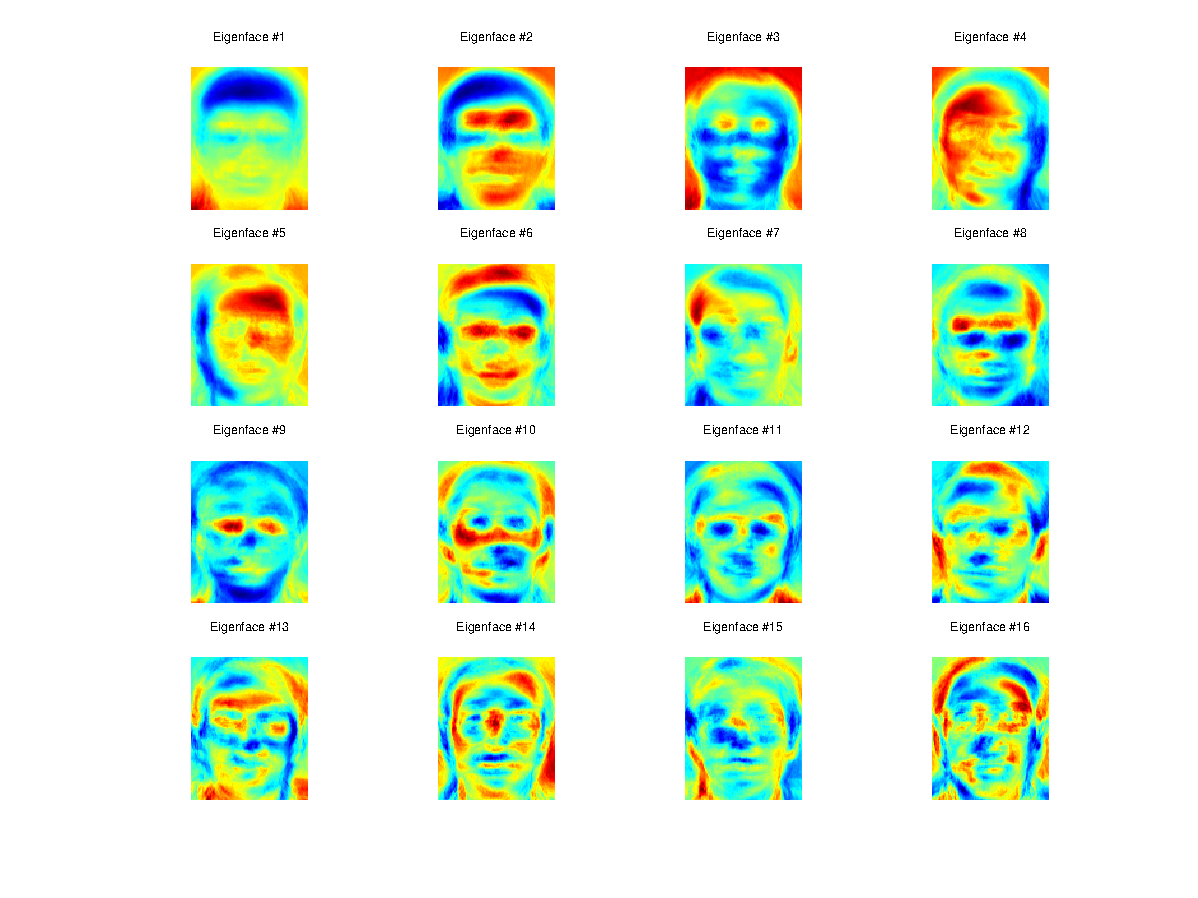
\includegraphics[scale=0.6]{img/eigenfaces/octave_pca_eigenfaces}
\end{center}
\else
	\begin{center}
		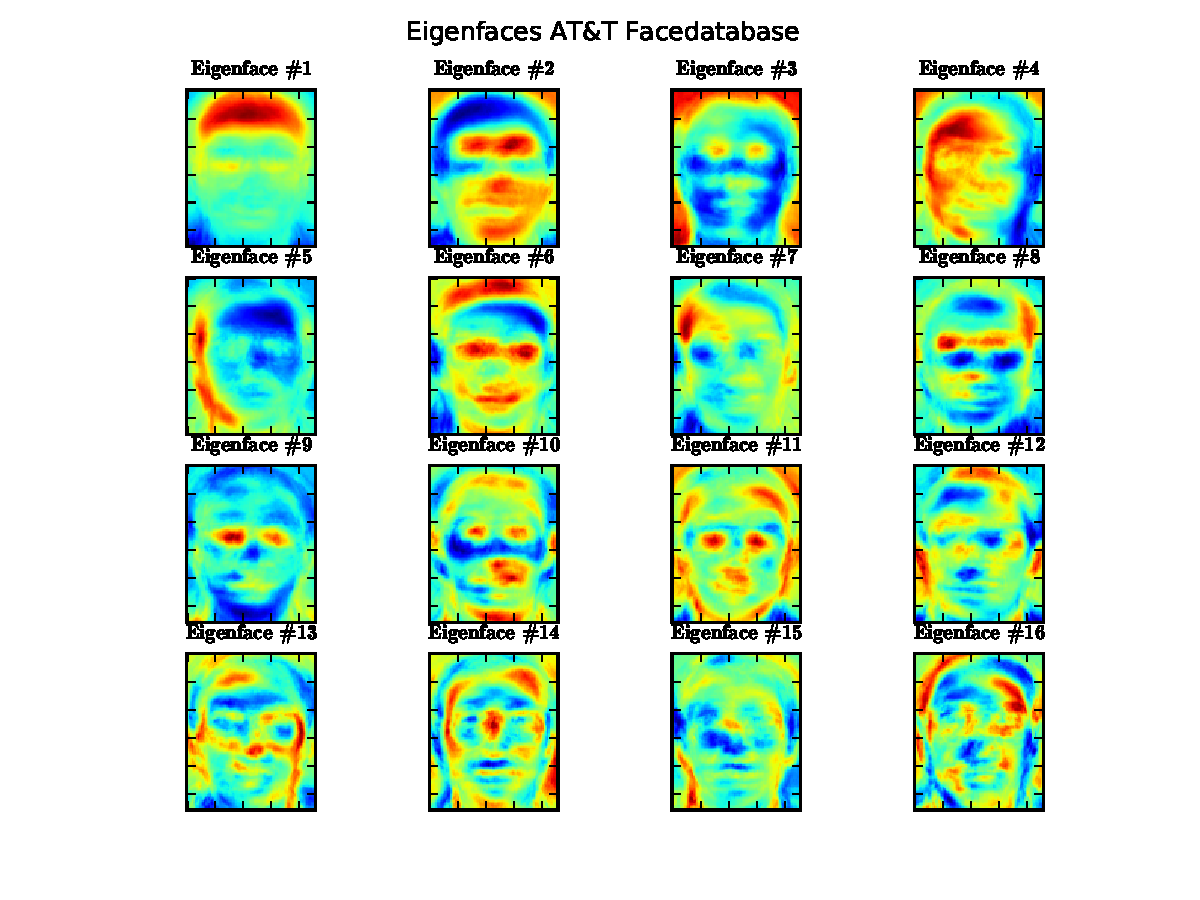
\includegraphics[scale=0.6]{img/eigenfaces/python_pca_eigenfaces}
	\end{center}
\fi

We've already seen in Equation \ref{eqn:pca_reconstruction}, that we can reconstruct a face from its lower dimensional approximation. So let's see how many Eigenfaces are needed for a good reconstruction. I'll do a subplot with $10,30,\ldots,310$ Eigenfaces:

\ifx\python\undefined
	\lstinputlisting[caption={\href{src/m/example\_eigenfaces.m}{src/m/example\_eigenfaces.m} \label{lst:example_pca3}}, language=matlab, linerange={23-36}]{src/m/example_eigenfaces.m}
\else
	\lstinputlisting[caption={\href{src/py/scripts/example\_pca.py}{src/py/scripts/example\_pca.py} \label{lst:example_pca3}}, language=python, linerange={27-40}]{src/py/scripts/example_pca.py}
\fi

10 Eigenvectors are obviously not sufficient for a good image reconstruction, 50 Eigenvectors may already be sufficient to encode important facial features. You'll get a good reconstruction with approximately 300 Eigenvectors for the AT\&T Facedatabase. There are rule of thumbs how many Eigenfaces you should choose for a successful face recognition, but it heavily depends on the input data. \cite{zhao2003frl} is the perfect point to start researching for this.

\ifx\python\undefined
	\begin{center}
		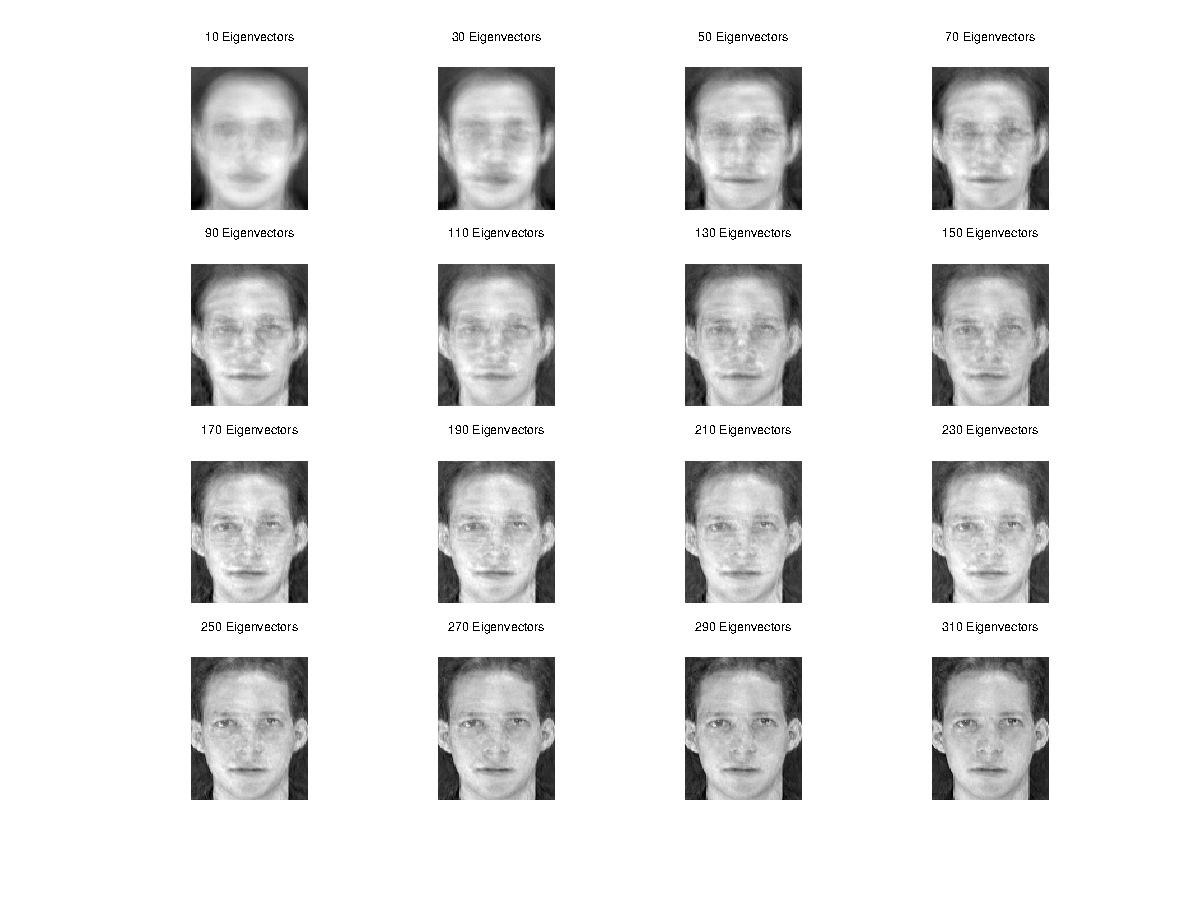
\includegraphics[scale=0.6]{img/eigenfaces/octave_pca_reconstruction}
	\end{center}
\else
	\begin{center}
		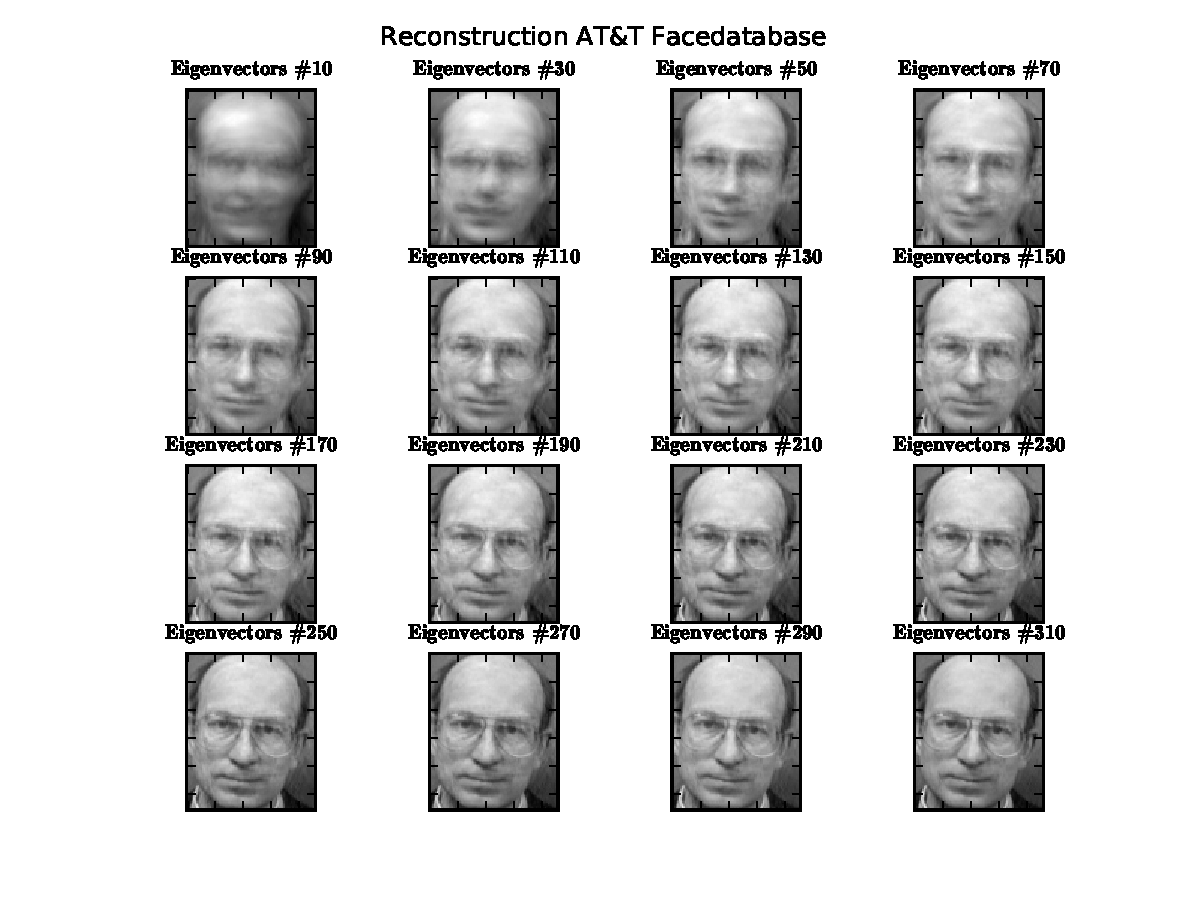
\includegraphics[scale=0.6]{img/eigenfaces/python_pca_reconstruction}
	\end{center}
\fi

\ifx\python\undefined
	The k-Nearest Neighbor matching is left out for this example. Please see the GNU Octave/MATLAB code at \url{https://github.com/bytefish/facerec/tree/master/m} to see how it is implemented, it's all there.
\else
	Now we have got everything to implement the Eigenfaces method. \href{http://www.python.org}{Python} is object oriented and so is our Eigenfaces model. Let's recap: The Eigenfaces method is basically a Pricipal Component Analysis with a Nearest Neighbor model. Some publications report about the influence of the distance metric (I can't support these claims with my research), so various distance metrics for the Nearest Neighbor should be supported. Listing \ref{lst:distance_base} defines an \lstinline|AbstractDistance| as the abstract base class for each distance metric. Every subclass overrides the call operator \lstinline|__call__| as shown for the Euclidean Distance and the Negated Cosine Distance. If you need more distance metrics, please have a look at the distance metrics implemented in \url{https://www.github.com/bytefish/facerec}.
	
	\lstinputlisting[caption={\href{src/py/tinyfacerec/distance.py}{src/py/tinyfacerec/distance.py} \label{lst:distance_base}}, language=python]{src/py/tinyfacerec/distance.py}
	
	The Eigenfaces and Fisherfaces method both share common methods, so we'll define a base prediction model in Listing \ref{lst:eigenfaces_base_model}. I don't want to do a full k-Nearest Neighbor implementation here, because (1) the number of neighbors doesn't really matter for both methods and (2) it would confuse people. If you are implementing it in a language of your choice, you should really separate the feature extraction and classification from the model itself. A real generic approach is given in my \href{https://www.github.com/bytefish/facerec}{facerec} framework. However, feel free to extend these basic classes for your needs.
	
	\lstinputlisting[caption={\href{src/py/tinyfacerec/model.py}{src/py/tinyfacerec/model.py} \label{lst:eigenfaces_base_model}}, language=python, linerange={1-28}]{src/py/tinyfacerec/model.py}

	Listing \ref{lst:eigenfaces_eigenfaces_model} then subclasses the \lstinline|EigenfacesModel| from the \lstinline|BaseModel|, so only the \lstinline|compute| method needs to be overriden with our specific feature extraction. The prediction is a 1-Nearest Neighbor search with a distance metric. 
	
	\lstinputlisting[caption={\href{src/py/tinyfacerec/model.py}{src/py/tinyfacerec/model.py} \label{lst:eigenfaces_eigenfaces_model}}, language=python, linerange={30-41}]{src/py/tinyfacerec/model.py}
	
		Now that the \lstinline|EigenfacesModel| is defined, it can be used to learn the Fisherfaces and generate predictions. In the following Listing \ref{lst:example_model_eigenfaces} we'll load the Yale Facedatabase A and perform a prediction on the first image.
		
	\lstinputlisting[caption={\href{src/py/scripts/example\_model\_eigenfaces.py}{src/py/scripts/example\_model\_eigenfaces.py} \label{lst:example_model_eigenfaces}}, language=python]{src/py/scripts/example_model_eigenfaces.py}

\fi

\subsection{Fisherfaces}

\label{ssection:fisherfaces}

The Linear Discriminant Analysis was invented by the great statistician \href{http://en.wikipedia.org/wiki/Ronald_Fisher}{Sir R. A. Fisher}, who successfully used it for classifying flowers in his 1936 paper \textit{The use of multiple measurements in taxonomic problems} \cite{Fisher36}. But why do we need another dimensionality reduction method, if the Principal Component Analysis (PCA) did such a good job? 

The PCA finds a linear combination of features that maximizes the total variance in data. While this is clearly a powerful way to represuccsent data, it doesn't consider any classes and so a lot of discriminative information may be lost when throwing components away. Imagine a situation where the variance is generated by an external source, let it be the light. The components identified by a PCA do not necessarily contain any discriminative information at all, so the projected samples are smeared together and a classification becomes impossible.

In order to find the combination of features that separates best between classes the Linear Discriminant Analysis maximizes the ratio of between-classes to within-classes scatter. The idea is simple: same classes should cluster tightly together, while different classes are as far away as possible from each other. This was also recognized by \href{http://www.cs.columbia.edu/~belhumeur/}{Belhumeur}, \href{http://www.ece.ucsb.edu/~hespanha/}{Hespanha} and \href{http://cseweb.ucsd.edu/~kriegman/}{Kriegman} and so they applied a Discriminant Analysis to face recognition in \cite{belhumeru97}. 

\begin{figure}
	\begin{center}
		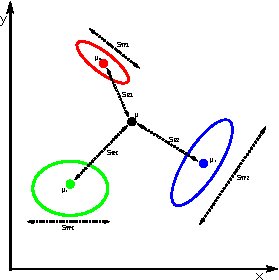
\includegraphics[scale=1.70]{img/fisherfaces/multiclasslda}
		\captionof{figure}{This figure shows the scatter matrices $S_{B}$ and $S_{W}$ for a 3 class problem. $\mu$ represents the total mean and $[\mu_{1},\mu_{2},\mu_{3}]$ are the class means.}
		\label{fig:scatter_matrices}
	\end{center}
\end{figure}

\subsubsection{Algorithmic Description}

Let $X$ be a random vector with samples drawn from $c$ classes:

\begin{eqnarray}
X & = & \{X_1,X_2,\ldots,X_c\} \\
X_i & = & \{x_1, x_2, \ldots, x_n\}
\end{eqnarray}

The scatter matrices $S_{B}$ and $S_{W}$ are calculated as:

% between-classes scatter
\begin{eqnarray}
\label{eqn:scatter_matrices}
S_{B} & = & \sum_{i=1}^{c} N_{i} (\mu_i - \mu)(\mu_i - \mu)^{T} \\
S_{W} & = & \sum_{i=1}^{c} \sum_{x_{j} \in X_{i}} (x_j - \mu_i)(x_j - \mu_i)^{T}
\end{eqnarray}

, where $\mu$ is the total mean:

\begin{equation}
\mu = \frac{1}{N} \sum_{i=1}^{N} x_i
\end{equation}

And $\mu_i$ is the mean of class $i \in \{1,\ldots,c\}$:

% Class-Average
\begin{equation}
\mu_i = \frac{1}{|X_i|} \sum_{x_j \in X_i} x_j
\end{equation}

Fisher's classic algorithm now looks for a projection $W$, that maximizes the class separability criterion:

\begin{equation}
W_{opt} = \operatorname{arg\,max}_{W} \frac{|W^T S_B W|}{|W^T S_W W|}
\end{equation}

Following \cite{belhumeru97}, a solution for this optimization problem is given by solving the General Eigenvalue Problem:

\begin{eqnarray}
\label{eqn:general_eigenwert}
S_{B} v_{i} & = & \lambda_{i} S_w v_{i} \nonumber \\
S_{W}^{-1} S_{B} v_{i} & = & \lambda_{i} v_{i}
\end{eqnarray}

There's one problem left to solve: The rank of $S_{W}$ is at most $(N-c)$, with $N$ samples and $c$ classes. In pattern recognition problems the number of samples $N$ is almost always samller than the dimension of the input data (the number of pixels), so the scatter matrix $S_{W}$ becomes singular (see \cite{Raudys1991}). In \cite{belhumeru97} this was solved by performing a Principal Component Analysis on the data and projecting the samples into the $(N-c)$-dimensional space. A Linear Discriminant Analysis was then performed on the reduced data, because $S_{W}$ isn't singular anymore.

The optimization problem can be rewritten as:

\begin{eqnarray}
W_{pca} & = & \operatorname{arg\,max}_{W} |W^T S_T W| \\
W_{fld} & = & \operatorname{arg\,max}_{W} \frac{|W^T W_{pca}^T S_{B} W_{pca} W|}{|W^T W_{pca}^T S_{W} W_{pca} W|}
\end{eqnarray}

The transformation matrix $W$, that projects a sample into the $(c-1)$-dimensional space is then given by:

\begin{equation} \label{eqn:fisherfaces}
W = W_{fld}^{T} W_{pca}^{T}
\end{equation}

One final note: Although $S_{W}$ and $S_{B}$ are symmetric matrices, the product of two symmetric matrices is not necessarily symmetric. so you have to use an eigenvalue solver for general matrices. OpenCV's \href{http://opencv.willowgarage.com/documentation/cpp/operations_on_arrays.html#cv-eigen}{cv::eigen} only works for symmetric matrices in its current version; since eigenvalues and singular values aren't equivalent for non-symmetric matrices you can't use a Singular Value Decomposition (SVD) either.

\ifx\python\undefined 
	\subsubsection{Fisherfaces in GNU Octave/MATLAB}
\else
 \subsubsection{Fisherfaces in Python}
\fi

\label{ssection:example_fisherfaces}

Translating the Linear Discriminant Analysis to \ifx\python\undefined \href{http://www.gnu.org/software/octave/}{GNU Octave}/\href{http://www.mathworks.com}{MATLAB} \else \href{http://www.python.org}{Python}\fi is almost trivial again, see Listing \ref{lst:lda}. For projecting and reconstructing from the basis you can use the functions from Listing \ref{lst:project} and \ref{lst:reconstruct}.
\ifx\python\undefined
	\lstinputlisting[caption={\href{src/m/lda.m}{src/m/lda.m} \label{lst:lda}}, language=matlab]{src/m/lda.m}
\else
		\lstinputlisting[caption={\href{src/py/tinyfacerec/subspace.py}{src/py/tinyfacerec/subspace.py} \label{lst:lda}}, language=python, linerange={39-58}]{src/py/tinyfacerec/subspace.py}
\fi

The functions to perform a PCA (Listing \ref{lst:pca}) and LDA (Listing \ref{lst:lda}) are now defined, so we can go ahead and implement the Fisherfaces from Equation \ref{eqn:fisherfaces}. 

\ifx\python\undefined
	\lstinputlisting[caption={\href{src/m/fisherfaces.m}{src/m/fisherfaces.m} \label{lst:fisherfaces}}, language=matlab]{src/m/fisherfaces.m}
\else
	\lstinputlisting[caption={\href{src/py/tinyfacerec/subspace.py}{src/py/tinyfacerec/subspace.py} \label{lst:fisherfaces}}, language=python, linerange={60-67}]{src/py/tinyfacerec/subspace.py}
\fi

For this example I am going to use the Yale Facedatabase A, just because the plots are nicer. Each Fisherface has the same length as an original image, thus it can be displayed as an image. We'll again load the data, learn the Fisherfaces and make a subplot of the first 16 Fisherfaces.

\ifx\python\undefined
	\lstinputlisting[caption={\href{src/m/example\_fisherfaces.m}{src/m/example\_fisherfaces.m} \label{lst:example_fisherfaces_fisherfaces}}, language=matlab, linerange={1-23}]{src/m/example_fisherfaces.m}
\else
	\lstinputlisting[caption={\href{src/py/scripts/example\_fisherfaces.py}{src/py/scripts/example\_fisherfaces.py} \label{lst:example_fisherfaces_fisherfaces}}, language=python, linerange={1-23}]{src/py/scripts/example_fisherfaces.py}
\fi

The Fisherfaces method learns a class-specific transformation matrix, so the they do not capture illumination as obviously as the Eigenfaces method. The Discriminant Analysis instead finds the facial features to discriminate between the persons. It's important to mention, that the performance of the Fisherfaces heavily depends on the input data as well. Practically said: if you learn the Fisherfaces for well-illuminated pictures only and you try to recognize faces in bad-illuminated scenes, then method is likely to find the wrong components (just because those features may not be predominant on bad illuminated images). This is somewhat logical, since the method had no chance to learn the illumination.

\ifx\python\undefined
	\begin{center}
		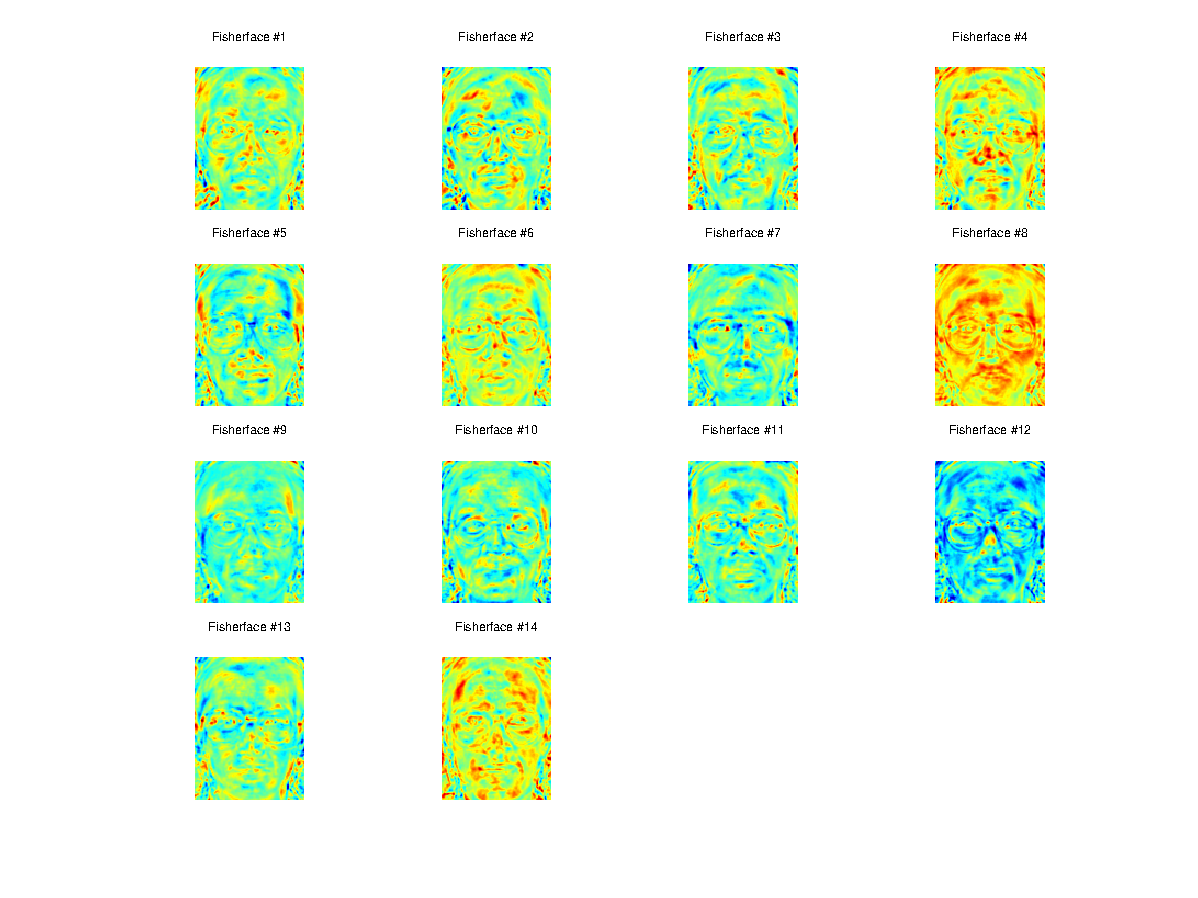
\includegraphics[scale=0.6]{img/fisherfaces/octave_fisherfaces_fisherfaces}
	\end{center}
\else
	\begin{center}
		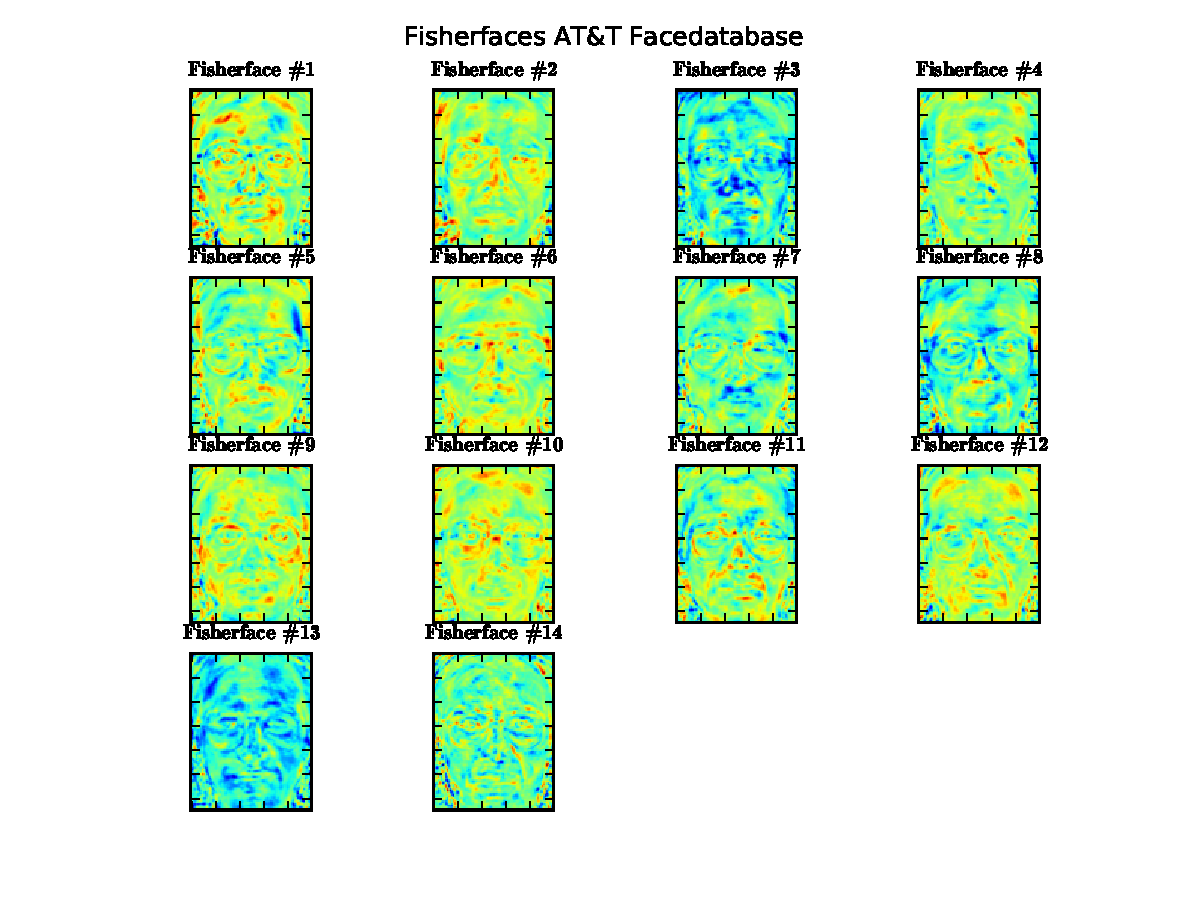
\includegraphics[scale=0.6]{img/fisherfaces/python_fisherfaces_fisherfaces}
	\end{center}
\fi

The Fisherfaces allow a reconstruction of the projected image, just like the Eigenfaces did. But since we only identified the features to distinguish between subjects, you can't expect a nice approximation of the original image. We can rewrite Listing \ref{lst:example_pca3} for the Fisherfaces method into Listing \ref{lst:example_fisherfaces_reconstruction}, but this time we'll project the sample image onto each of the Fisherfaces instead. So you'll have a visualization, which features each Fisherface describes.

\ifx\python\undefined
	\lstinputlisting[caption={\href{src/m/example\_fisherfaces.m}{src/m/example\_fisherfaces.m} \label{lst:example_fisherfaces_reconstruction}}, language=matlab, linerange={28-40}]{src/m/example_fisherfaces.m}
\else
	\lstinputlisting[caption={\href{src/py/scripts/example\_fisherfaces.py}{src/py/scripts/example\_fisherfaces.py} \label{lst:example_fisherfaces_reconstruction}}, language=python, linerange={25-36}]{src/py/scripts/example_fisherfaces.py}
\fi


\ifx\python\undefined
	\begin{center}
		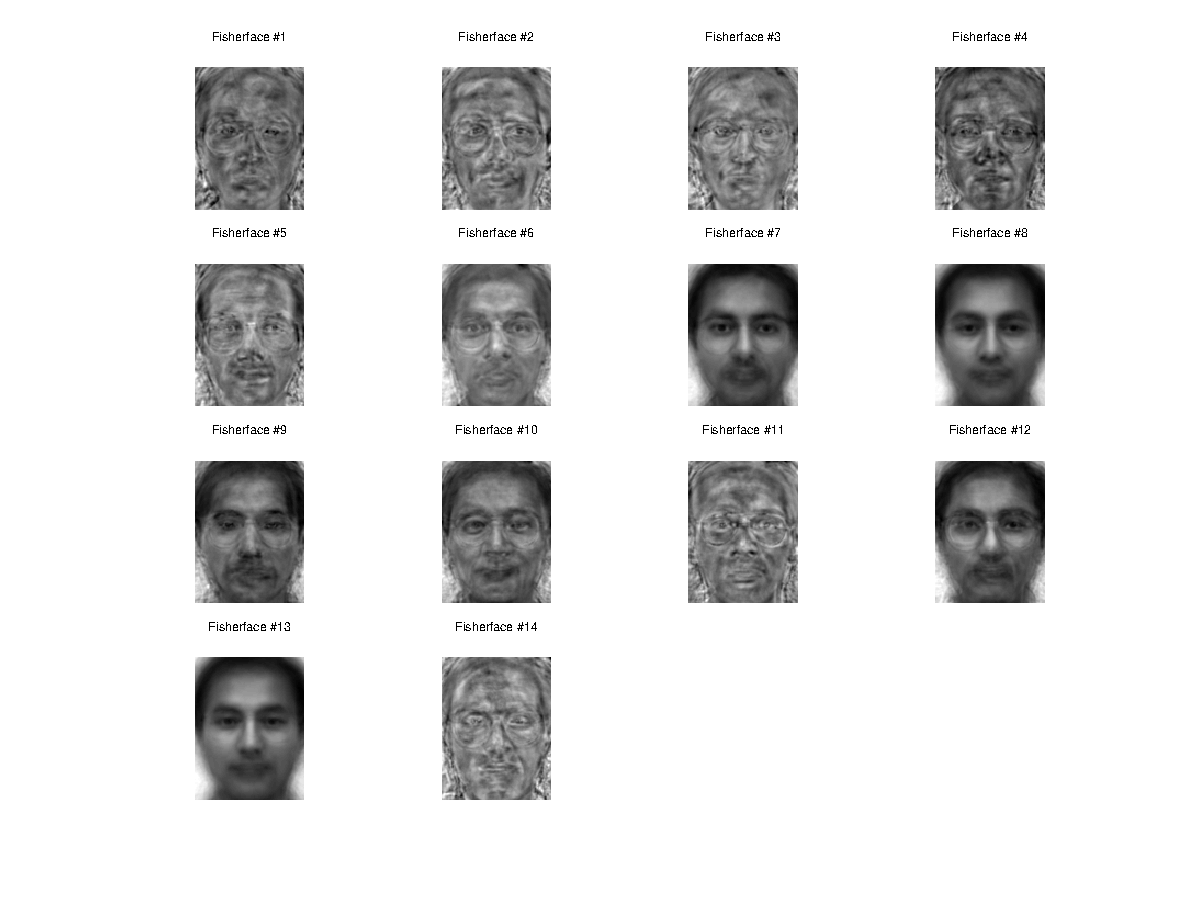
\includegraphics[scale=0.6]{img/fisherfaces/octave_fisherfaces_reconstruction}
	\end{center}
\else
	\begin{center}
		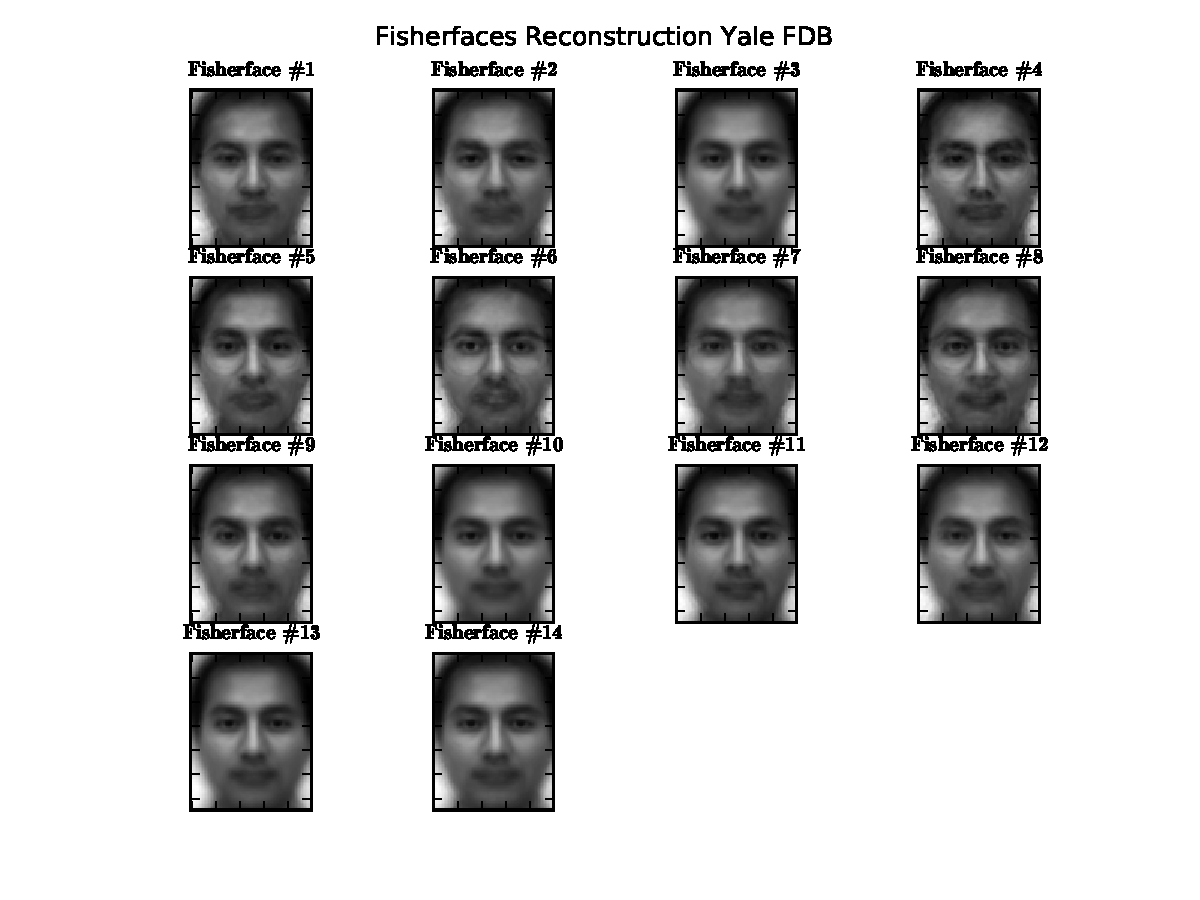
\includegraphics[scale=0.6]{img/fisherfaces/python_fisherfaces_reconstruction}
	\end{center}
\fi

\ifx\python\undefined
	The k-Nearest Neighbor matching is left out for this example. Please see the GNU Octave/MATLAB code at \url{https://github.com/bytefish/facerec/tree/master/m} to see how it is implemented, it's all there.
\else
	The implementation details are not repeated in this section. For the Fisherfaces method a similar model to the \lstinline|EigenfacesModel| in Listing \ref{lst:eigenfaces_eigenfaces_model} must be defined.
		
	\lstinputlisting[caption={\href{src/py/tinyfacerec/model.py}{src/py/tinyfacerec/model.py} \label{lst:eigenfaces_eigenfaces_model}}, language=python, linerange={43-54}]{src/py/tinyfacerec/model.py}
	
		Once the \lstinline|FisherfacesModel| is defined, it can be used to learn the Fisherfaces and generate predictions. In the following Listing \ref{lst:example_model_fisherfaces} we'll load the Yale Facedatabase A and perform a prediction on the first image.
		
	\lstinputlisting[caption={\href{src/py/scripts/example\_model\_fisherfaces.py}{src/py/scripts/example\_model\_fisherfaces.py} \label{lst:example_model_fisherfaces}}, language=python]{src/py/scripts/example_model_fisherfaces.py}

\fi


